% !TeX root = ../thesis.tex
%================1.7

\section{Minh họa phân loại một chiều trên bộ dữ liệu hoa diên vỹ (Iris Dataset)}

Để minh họa cụ thể quy tắc phân loại tuyến tính trong trường hợp một chiều, ta xét bộ dữ liệu Iris của Fisher. Bộ dữ liệu này gồm ba loài hoa Iris là \textit{setosa}, \textit{versicolor} và \textit{virginica}, với bốn thuộc tính đo lường hình thái học: chiều dài đài hoa \textit{Sepal.Length}, chiều rộng đài hoa \textit{Sepal.Width}, chiều dài cánh hoa \textit{Petal.Length} và chiều rộng cánh hoa \textit{Petal.Width}. Các thuộc tính này đều được đo bằng đơn vị centimet, ký hiệu là \(\text{cm}\). Bộ dữ liệu Iris gồm tổng cộng \(150\) quan sát, trong đó mỗi loài hoa có \(50\) quan sát. Cụ thể,
\[
n_{\textit{setosa}}=n_{\textit{versicolor}}=n_{\textit{virginica}}=50.
\]
Một phần dữ liệu Iris được minh họa thông qua 6 quan sát đầu tiên như trong bảng sau
\begin{table}[H]
	\centering
	\small
	\begin{tabular}{|c|ccccc|}
		\hline
		STT & Sepal.Length & Sepal.Width & Petal.Length & Petal.Width & Species \\ \hline
		1 & 5{,}1 & 3{,}5 & 1{,}4 & 0{,}2 & setosa \\
		2 & 4{,}9 & 3{,}0 & 1{,}4 & 0{,}2 & setosa \\
		3 & 4{,}7 & 3{,}2 & 1{,}3 & 0{,}2 & setosa \\
		4 & 4{,}6 & 3{,}1 & 1{,}5 & 0{,}2 & setosa \\
		5 & 5{,}0 & 3{,}6 & 1{,}4 & 0{,}2 & setosa \\
		6 & 5{,}4 & 3{,}9 & 1{,}7 & 0{,}4 & setosa \\ \hline
	\end{tabular}
	\caption{6 quan sát đầu tiên của bộ dữ liệu Iris.}
	\label{tab:SauDongDauIris}
\end{table}

Hình \ref{fig:iris_petal_length_width} biểu diễn đám mây điểm của ba lớp hoa Iris theo hai thuộc tính \textit{Petal.Length} và \textit{Petal.Width}. Qua hình này, ta thấy lớp \textit{setosa} được tách biệt khá rõ so với hai lớp còn lại, trong khi hai lớp \textit{versicolor} và \textit{virginica} có vùng gần nhau hơn.

\begin{figure}[H]
	\centering
	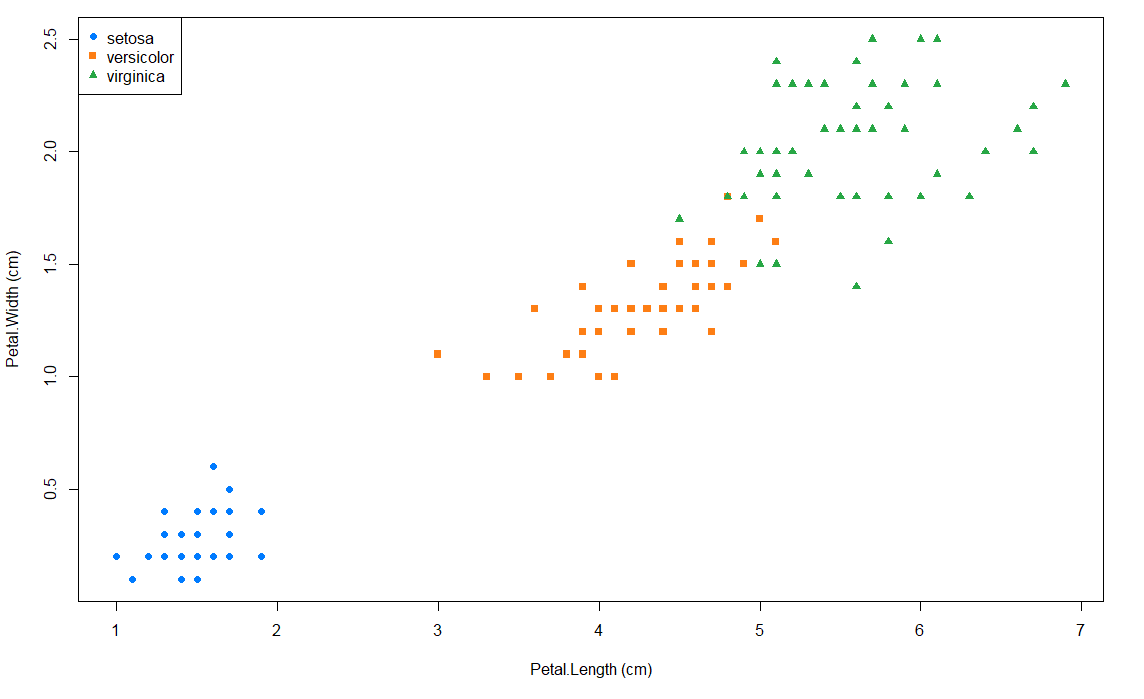
\includegraphics[width=0.85\textwidth]{image/iris_test.png}
	\caption{Đám mây điểm của ba lớp trong bộ dữ liệu Iris theo hai thuộc tính \textit{Petal.Length} và \textit{Petal.Width}.}
	\label{fig:iris_petal_length_width}
\end{figure}
Trong ví dụ này, ta chỉ xét hai lớp hoa
\[
C_1=\textit{versicolor}, \qquad C_2=\textit{virginica},
\]
và chỉ sử dụng một thuộc tính duy nhất là chiều dài cánh hoa, ký hiệu bởi
\[
x=\text{Petal.Length}.
\]
Như vậy, bài toán phân loại nhiều chiều ban đầu được rút gọn thành bài toán phân loại một chiều trên trục thực.

Gọi $\textbf{x}_1$ là tập các quan sát thuộc lớp \textit{versicolor} và $\textbf{x}_2$ là tập các quan sát thuộc lớp \textit{virginica}. Từ dữ liệu Iris, ta có
\[
n_1=n_2=50,
\]
do đó xác suất tiên nghiệm của hai lớp là
\[
\hat\pi_1=\hat\pi_2=\frac{1}{2}.
\]

Trung bình mẫu của thuộc tính \textit{Petal.Length} trong hai lớp lần lượt là
\[
\hat{\mu}_1 = 4{,}260\ (\text{cm}), \qquad
\hat{\mu}_2 = 5{,}552\ (\text{cm}).
\]
Phương sai mẫu của hai lớp là
\[
s_1^2 = 0{,}2208\ (\text{cm}^2), \qquad
s_2^2 = 0{,}3046\ (\text{cm}^2).
\]
Vì LDA giả thiết hai lớp có chung phương sai trong trường hợp một chiều, phương sai gộp được ước lượng bởi
\[
s_p^2=
\frac{(n_1-1)s_1^2+(n_2-1)s_2^2}{n_1+n_2-2}.
\]
Thay số vào ta được
\[
s_p^2
=
\frac{49(0{,}2208)+49(0{,}3046)}{98}
\approx 0{,}2627\;(\text{cm}^2).
\]

Trong trường hợp một chiều, hàm tách biệt LDA của lớp $k$ có dạng
\[
\hat\delta_k(x)
=
x\frac{\hat\mu_k}{s_p^2}
-
\frac{1}{2}\frac{\hat\mu_k^2}{s_p^2}
+
\ln \hat\pi_k,
\qquad k=1,2.
\]
Biên quyết định giữa hai lớp được xác định bởi điều kiện
\[
\hat{\delta}_1(x)=\hat{\delta}_2(x).
\]
Giải phương trình này theo $x$, ta thu được ngưỡng phân loại
\[
x_{\text{bnd}}
=
\frac{\hat\mu_1+\hat\mu_2}{2}
-
\frac{s_p^2}{\hat\mu_2-\hat\mu_1}
\ln\frac{\hat\pi_2}{\hat\pi_1}.
\]
Trong ví dụ này, do hai lớp có cùng số quan sát nên
\[
\hat\pi_1=\hat\pi_2,
\]
suy ra
\[
\ln\frac{\hat\pi_2}{\hat\pi_1}=0.
\]
Vì vậy, ngưỡng phân loại trở thành trung điểm giữa hai trung bình
\[
x_{\text{bnd}}
=
\frac{\hat{\mu}_1+\hat{\mu}_2}{2}
=
\frac{4{,}260+5{,}552}{2}
=
4{,}906\;(\text{cm}).
\]

Do $\hat\mu_2>\hat\mu_1$, quy tắc phân loại LDA trong trường hợp này là
\[
\hat G(x)=
\begin{cases}
	C_1, & x \leq 4{,}906\;(\text{cm}),\\
	C_2, & x > 4{,}906\;(\text{cm}).
\end{cases}
\]
Hay viết cụ thể theo tên loài hoa
\[
\hat G(x)=
\begin{cases}
	\textit{versicolor}, & \text{nếu } \text{Petal.Length}\leq 4{,}906\;(\text{cm}),\\
	\textit{virginica}, & \text{nếu } \text{Petal.Length}>4{,}906\;(\text{cm}).
\end{cases}
\]

Hình~\ref{fig:lda_iris_1d} biểu diễn hai mật độ Gaussian một chiều được ước lượng từ dữ liệu của hai lớp \textit{versicolor} và \textit{virginica}. Hai đường cong được vẽ dưới dạng $\hat\pi_k f_k(x)$, tức là mật độ nhân với xác suất tiên nghiệm của lớp tương ứng. Đường thẳng đứng nét đứt màu đen biểu diễn ngưỡng phân loại LDA tại $x_{\text{bnd}}=4{,}906\;(\text{cm})$.

\begin{figure}[H]
	\centering
	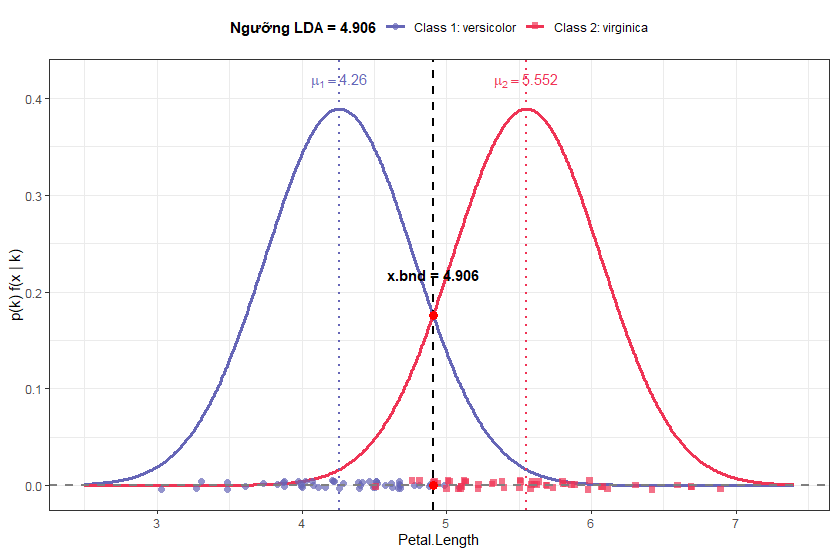
\includegraphics[width=0.85\textwidth]{image/bayes1D.png}
	\caption{Minh họa phân loại một chiều bằng LDA trên bộ dữ liệu Iris với hai lớp \textit{versicolor} và \textit{virginica} theo thuộc tính \textit{Petal.Length}.}
	\label{fig:lda_iris_1d}
\end{figure}

Từ hình minh họa có thể thấy phân phối của lớp \textit{versicolor} tập trung chủ yếu về phía bên trái, trong khi phân phối của lớp \textit{virginica} tập trung về phía bên phải. Tuy nhiên, hai phân phối vẫn có một vùng chồng lấn xung quanh ngưỡng phân loại. Đây chính là vùng mà khả năng phân loại sai có thể xảy ra.

Kết quả phân loại trên 100 quan sát thuộc hai lớp cho ma trận lỗi như sau
\[
\begin{array}{c|cc}
	& \text{versicolor} & \text{virginica} \\
	\hline
	\text{Dự đoán versicolor} & 48 & 6 \\
	\text{Dự đoán virginica} & 2 & 44
\end{array}
\]
Do đó, số quan sát bị phân loại sai là
\[
2+6=8.
\]
Tỷ lệ phân loại sai là
\[
\frac{8}{100}=0{,}08=8\%.
\]
Như vậy, trong ví dụ một chiều này, bộ phân loại LDA đạt tỷ lệ lỗi xấp xỉ $8\%$.
Ví dụ trên cho thấy khi giả thiết hai lớp có phân phối Gaussian với cùng phương sai, biên quyết định LDA trong không gian một chiều chỉ là một điểm cắt trên trục số. Các quan sát nằm về một phía của điểm cắt được gán vào lớp thứ nhất, còn các quan sát nằm về phía còn lại được gán vào lớp thứ hai. Đây là dạng đơn giản nhất của biên tuyến tính trong LDA.

\hspace*{0.5cm}Ở ví dụ trước, hai lớp \textit{versicolor} và \textit{virginica} có vùng giao nhau nên LDA vẫn có thể phát sinh lỗi phân loại. Để minh họa trường hợp biên quyết định một chiều có thể phân tách hoàn toàn dữ liệu, ta xét một cặp hoa khác trong bộ dữ liệu Iris, đó là \textit{setosa} và \textit{versicolor}, tiếp tục với thuộc tính phân loại là \textit{Petal.Length}.

Gọi
\[
C_1=\textit{setosa}, \qquad C_2=\textit{versicolor},
\]
và
\[
x=\text{Petal.Length}.
\]
Khi đó, mỗi quan sát được biểu diễn bởi một giá trị thực trên trục một chiều.

Từ bộ dữ liệu Iris, mỗi lớp có 50 quan sát, do đó
\[
n_1=n_2=50.
\]
Suy ra xác suất tiên nghiệm của hai lớp là
\[
\hat{\pi}_1=\hat{\pi}_2=\frac{1}{2}.
\]

Trung bình mẫu của thuộc tính \textit{Petal.Length} trong hai lớp lần lượt là
\[
\hat{\mu}_1=1{,}462\;(\text{cm}), 
\qquad 
\hat{\mu}_2=4{,}260\;(\text{cm}).
\]
Trong đó, $\hat{\mu}_1$ là trung bình của lớp \textit{setosa}, còn $\hat{\mu}_2$ là trung bình của lớp \textit{versicolor}. Phương sai mẫu tương ứng là
\[
s_1^2=0{,}0302\;(\text{cm}^2), 
\qquad 
s_2^2=0{,}2208\;(\text{cm}^2).
\]

Phương sai gộp được tính bởi
\[
s_p^2
=
\frac{(n_1-1)s_1^2+(n_2-1)s_2^2}{n_1+n_2-2}.
\]
Thay số vào ta được
\[
s_p^2
=
\frac{49(0{,}0302)+49(0{,}2208)}{98}
\approx
0{,}1255\;(\text{cm}^2).
\]

Trong trường hợp một chiều, hàm tách biệt LDA của lớp $k$ có dạng
\[
\hat{\delta}_k(x)
=
x\frac{\hat{\mu}_k}{s_p^2}
-
\frac{1}{2}\frac{\hat{\mu}_k^2}{s_p^2}
+
\ln\hat{\pi}_k,
\qquad k=1,2.
\]
Biên quyết định giữa hai lớp được xác định bởi điều kiện
\[
\hat{\delta}_1(x)=\hat{\delta}_2(x).
\]
Giải phương trình trên theo $x$, ta thu được ngưỡng phân loại
\[
x_{\text{bnd}}
=
\frac{\hat{\mu}_1+\hat{\mu}_2}{2}
-
\frac{s_p^2}{\hat{\mu}_2-\hat{\mu}_1}
\ln\frac{\hat{\pi}_2}{\hat{\pi}_1}.
\]

Do hai lớp có cùng số quan sát nên
\[
\hat{\pi}_1=\hat{\pi}_2.
\]
Suy ra
\[
\ln\frac{\hat{\pi}_2}{\hat{\pi}_1}=0.
\]
Vì vậy, ngưỡng phân loại trở thành
\[
x_{\text{bnd}}
=
\frac{\hat{\mu}_1+\hat{\mu}_2}{2}
=
\frac{1{,}462+4{,}260}{2}
\approx
2{,}861\;(\text{cm}).
\]

Mặt khác, trong dữ liệu thực tế, giá trị lớn nhất của \textit{Petal.Length} đối với lớp \textit{setosa} là
\[
\max(\textit{setosa})=1{,}9\;(\text{cm}),
\]
trong khi giá trị nhỏ nhất của \textit{Petal.Length} đối với lớp \textit{versicolor} là
\[
\min(\textit{versicolor})=3{,}0\;(\text{cm}).
\]
Do đó
\[
1{,}9 < 3{,}0.
\]
Điều này cho thấy hai lớp \textit{setosa} và \textit{versicolor} được tách biệt hoàn toàn theo thuộc tính \textit{Petal.Length}. Khoảng trống giữa hai lớp là từ $1{,}9$ đến $3{,}0$ cm.

Ngưỡng LDA
\[
x_{\text{bnd}}\approx 2{,}861\;(\text{cm})
\]
nằm trong khoảng trống này, nên có thể phân loại đúng toàn bộ các quan sát thuộc hai lớp.

Do $\hat{\mu}_2>\hat{\mu}_1$, quy tắc phân loại LDA trong ví dụ này là
\[
\hat{G}(x)=
\begin{cases}
	\textit{setosa}, & \text{nếu } \text{Petal.Length}\leq 2{,}861\;(\text{cm}),\\
	\textit{versicolor}, & \text{nếu } \text{Petal.Length}>2{,}861\;(\text{cm}).
\end{cases}
\]

Hình~\ref{fig:lda_iris_setosa_versicolor} minh họa hai phân phối một chiều của hai lớp \textit{setosa} và \textit{versicolor} theo thuộc tính \textit{Petal.Length}. Đường thẳng đứng nét đứt màu đen biểu diễn ngưỡng phân loại LDA. Các điểm dữ liệu thực tế của hai lớp nằm ở hai phía khác nhau của ngưỡng, cho thấy sự tách biệt hoàn toàn trong trường hợp này.

\begin{figure}[H]
	\centering
	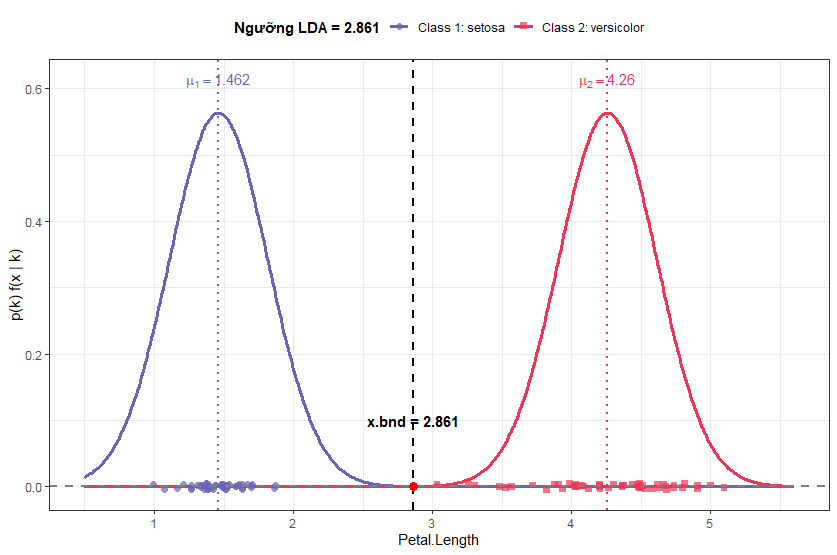
\includegraphics[width=0.85\textwidth]{image/bayes1Dgood.png}
	\caption{Minh họa phân loại một chiều bằng LDA trên bộ dữ liệu Iris với hai lớp \textit{setosa} và \textit{versicolor} theo thuộc tính \textit{Petal.Length}.}
	\label{fig:lda_iris_setosa_versicolor}
\end{figure}

Kết quả phân loại trên 100 quan sát thuộc hai lớp \textit{setosa} và \textit{versicolor} cho ma trận lỗi
\[
\begin{array}{c|cc}
	& \textit{setosa} & \textit{versicolor} \\
	\hline
	\text{Dự đoán setosa} & 50 & 0 \\
	\text{Dự đoán versicolor} & 0 & 50
\end{array}
\]
Từ ma trận trên, không có quan sát nào bị phân loại sai. Do đó, tỷ lệ lỗi phân loại là
\[
\frac{0}{100}=0.
\]

Ví dụ này cho thấy trong trường hợp một chiều, nếu hai lớp có sự tách biệt rõ ràng trên một thuộc tính, biên quyết định của LDA chỉ là một điểm cắt trên trục số và có thể phân loại hoàn toàn chính xác các quan sát trong dữ liệu. Trường hợp \textit{setosa} và \textit{versicolor} với thuộc tính \textit{Petal.Length} là một minh họa điển hình cho khả năng phân tách tuyến tính của LDA trong không gian một chiều.


